\documentclass[12pt]{article}
\usepackage{enumerate}
\usepackage{notes}
\usepackage{oxford}

\begin{document}

\section{2017}

\subsection*{}  % 1
\begin{mdframed}
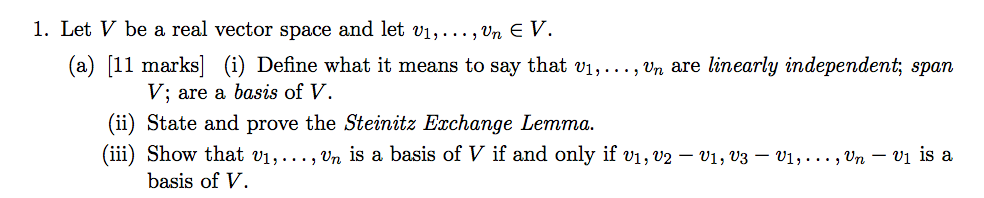
\includegraphics[width=400pt]{img/oxford-prelims-2017-A-1-1.png}
\end{mdframed}

\subsubsection*{(i)}
\begin{definition*}[Linear independence]
  Let $a_1, \ldots, a_n \in \R$. Then $v_1, v_2, \ldots, v_n$ are linearly
  independent if and only if the only solution to $\sum_{i=1}^n a_iv_i = 0$ is
  $a_1 = a_2 = \ldots = a_n = 0$.
\end{definition*}

\begin{definition*}[Span]
  $v_1, v_2, \ldots, v_n$ span $V$ if and only if for all $w \in V$ there exist
  $a_1, \ldots, a_n \in \R$ such that $\sum_{i=1}^n a_iv_i = w$.
\end{definition*}

\begin{definition*}[Basis]
  $v_1, v_2, \ldots, v_n$ are a basis for $V$ if and only if they span $V$ and
  they are linearly independent.
\end{definition*}

\subsubsection*{(ii)}

\begin{theorem*}[Steinitz Exchange Lemma]
  Let $V$ be a vector space, let $v_1, \ldots, v_n$ be a basis for $V$ and
  let $w_1, \ldots, w_m \in V$ be linearly independent, where $m \leq
  n$. Then, possibly after reordering the $v_i$,
  \begin{align*}
    w_1, \ldots, w_m, v_{m+1}, \ldots, v_n
  \end{align*}
  is also a basis for $V$.
\end{theorem*}

\begin{proof}
  Let $P(m)$ be the following proposition:

  It's true for $m = n$, since the dimension of $V$ is $n$, and therefore any
  collection of $n$ linearly independent vectors is a basis.

  Let $m = n - 1$. We want to show that there exists a $v_i$ that can be
  contributed to the $\{w_i\}$ without losing linear independence.

  The $\{w_i\}$ span a subspace $U$ of $V$, of dimension $m = n-1$.

  Let $v_n$ (after reordering the $\{v_i\}$) be an element of the basis that is
  not in $U$ (there exists at least one such $v_i$).


\end{proof}

\subsubsection*{(iii)}

$\implies$\\


$\impliedby$\\
Let $v_1, v_2 - v_1, \ldots, v_n - v_1$ be a basis of $V$.

Then for all $w \in V$ there exist $a_1, \ldots, a_n$, all non-zero, such that
\begin{align*}
  a_1v_1 + \sum_{i=2}^n a_i(v_i - v_1) = w.
\end{align*}
Therefore
\begin{align*}
  \Big(a_1 - \sum_{i=2}^na_i\Big)v_1 + \sum_{i=2}^n a_iv_i = w.
\end{align*}

So $v_1, v_2, \ldots, v_n$ span $V$ (TODO: but how do we know that $a_1 \neq \sum_{i=2}^na_i$?)

TODO: linear independence

~\\
\begin{mdframed}
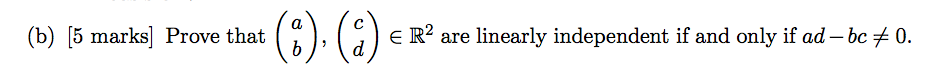
\includegraphics[width=400pt]{img/oxford-prelims-2017-A-1-2.png}
\end{mdframed}

~\\
\begin{mdframed}
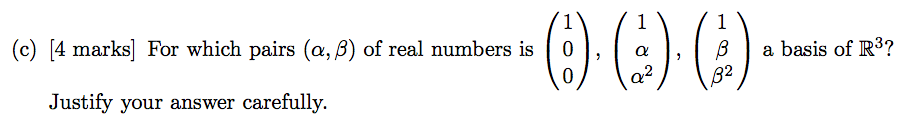
\includegraphics[width=400pt]{img/oxford-prelims-2017-A-1-3.png}
\end{mdframed}

~\\
\subsection*{}  % 2
\begin{mdframed}
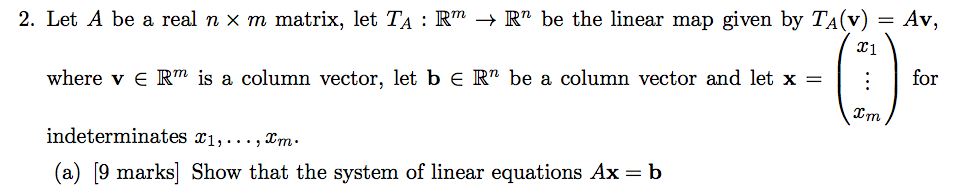
\includegraphics[width=400pt]{img/oxford-prelims-2017-A-2-1.png}
\end{mdframed}

\subsection*{}  % 2.a.i
\begin{mdframed}

\includegraphics[width=400pt]{img/oxford-prelims-2017-A-2-1-1.png}
\end{mdframed}

By definition,  $\Im T_A = \{Ax: x \in \R^m\}$.

Let $S$ denote the proposition ``$Ax = b$ has a solution''.

By the definition of ``has a solution'', $S$ is equivalent to the proposition
``there exists $x \in \R^m$ such that $Ax = b$''.

We see that $S \implies b \in \Im T_A$, and also that $b \in \Im T_A \implies S$.

% By definition, $\Im T_A = \{b : \exists x : Ax = b\}$, we then have $b \in \Im
% T_A$. Therefore $S \implies b \in \Im T_A$.

% Conversely if $b \in \Im T_A$ then

% ``$Ax = b$ has a solution'' is logically equivalent to ``$b \in \Im T_A$'' by
% the definitions of ``have a solution'' and $\Im$: they both mean ``there exists
% $x \in \R^m$ such that $Ax = b$''.

% The meaning of ``$Ax = b$ has a solution'' is: there exists $x \in \R^m$ such that
% $Ax = b$.

% If $b \in \Im T_A$ then, by definition of $\Im$, $Ax = b$ has a solution.

% Conversely, if $Ax = b$ has a solution, then $b \in \Im T_A$.

\subsubsection*{} % 2.a.ii
\begin{mdframed}
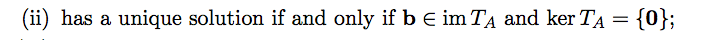
\includegraphics[width=400pt]{img/oxford-prelims-2017-A-2-1-2.png}
\end{mdframed}

Let $S_u$ denote the proposition ``$Ax = b$ has a unique solution''.

\begin{claim*}
  $S_u \implies \Big(b \in \Im T_A ~~\text{and}~~ \ker T_A = \{0\}\Big)$.
\end{claim*}

\begin{proof}
Firstly, since $S_u \implies S$, we know from part (i) that
$S_u \implies b \in \Im T_A$.

Suppose $S_u$ is true and let $x$ be the unique solution.

We know that $0 \in \ker A$ since $A(0) = A(x - x) = Ax - Ax = 0$ by the
linearity of $A$.

Now suppose there exists $y \neq 0 \in \ker T_A$. But
\begin{align*}
A(x + y) = Ax + Ay = b + 0 = b,
\end{align*}
so $x + y \neq x$ is also a solution; a contradiction. Therefore no such $y$
exists and we see that $S_u \implies \ker T_A = \{0\}$.
\end{proof}

\begin{claim*}
  $\Big(b \in \Im T_A ~~\text{and}~~ \ker T_A = \{0\}\Big) \implies S_u$.
\end{claim*}

\begin{proof}
  Suppose $b \in \Im T_A$. Then we know from part (i) that $S$ is true. So let
  $x$ be a solution.

Now suppose that $\ker T_A = \{0\}$ and that $y \neq x$ is another solution. But then
\begin{align*}
  A(x - y) = Ax - Ay = b - b = 0,
\end{align*}
so $x - y \neq 0 \in \ker T_A$; a contradition. Therefore if $\ker T_A = \{0\}$
then no such $y$ exists.
\end{proof}

\subsubsection*{} % 2.a.iii
\begin{mdframed}
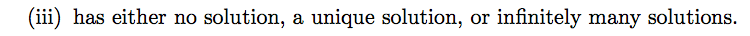
\includegraphics[width=400pt]{img/oxford-prelims-2017-A-2-1-3.png}
\end{mdframed}

Suppose $Ax = b$ has $n > 1$ solutions and let the first two such solutions be
$x_1$ and $x_2$. Then there are uncountably infinitely many solutions, since
for all $\alpha \in \R$
\begin{align*}
A\Big(x_1 + \alpha (x_2 - x_1)\Big) = Ax_1 + \alpha(Ax_2 - Ax_1) = b + \alpha(b - b) = b.
\end{align*}

~\\
\subsection*{} % 2.b
\begin{mdframed}
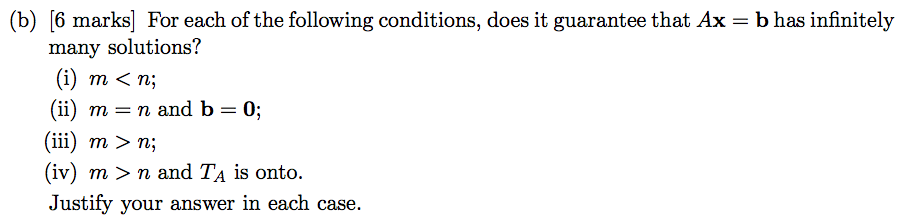
\includegraphics[width=400pt]{img/oxford-prelims-2017-A-2-2.png}
\end{mdframed}

\subsubsection*{(i)}

~\\
\subsection*{} % 2.c
\begin{mdframed}
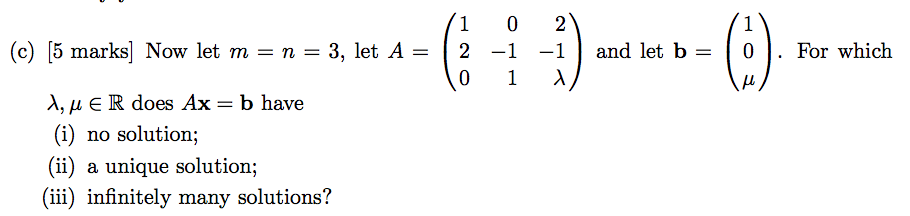
\includegraphics[width=400pt]{img/oxford-prelims-2017-A-2-3.png}
\end{mdframed}

\end{document}
